In this chapter we present our case study of the elevator system,
how the model is translated into variables and parameters and which
constraints we need in order to perform the configuration and the 
cost functions required to achieve design.

\section{Variables and Parameters}
\label{sec:variables}

We now introduce the decision variables and the parameters involved
in the configuration task. We note that the 
reference system in \liftcreate{} origins from the top left corner 
of the internal shaft wall and the $y$ axis is inverted with respect 
to a canonical Cartesian system. The origin $\mathcal{O}_{(x,y)}$ of 
this reference system coincides with the \emph{shaft base point} 
$(x_{shaft}, y_{shaft})$ which is always set to $(0, 0)$ --- see 
Fig.~\ref{img:planView}. 
%
\begin{figure}[t]
	\caption{\label{img:dpDetailView} Detail of the car/landing 
		door pair and related parameters.}
	\centering
	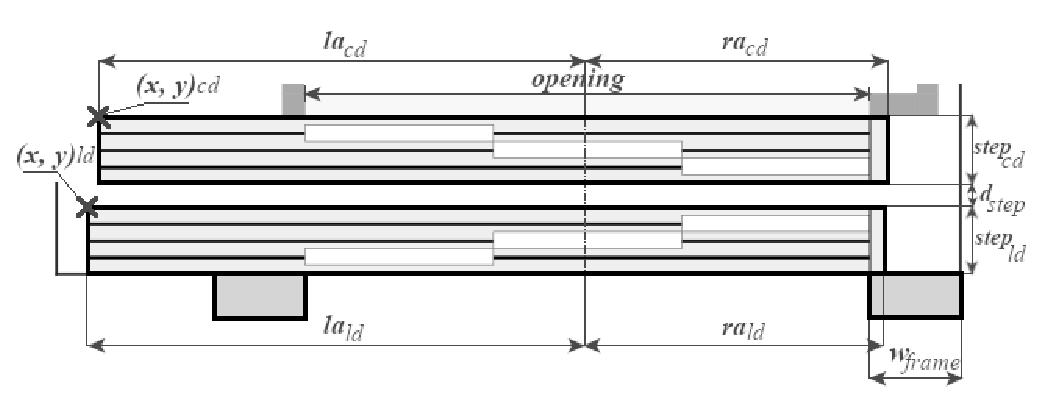
\includegraphics[width=.8\linewidth]{Elevator/DP.eps}
\end{figure}
%
In Fig.~\ref{img:cfDetailView} we 
present a fragment of the plan view focusing on the car frame structure, 
which is comprised of the \emph{brackets} --- wall-mounted T-shaped 
components --- to support the car rails on which the car frame 
\emph{core gear} slides. The \emph{car frame base point}, i.e., the 
insertion point of the car frame structure in the configuration, 
lies on the outer corner of the topmost bracket and it is marked with 
a cross. The coordinates of the car frame base point $(x_{cf},y_{cf})$ 
--- denoted by $(x,y)_{cf}$ in Fig.~\ref{img:cfDetailView} ---
determine a specific placement of the structure. The \emph{overhang}
of the car with respect to the car frame is the distance from the car
walls to the car frame core gear edges --- the top edge is $y_{gear}$.
As shown in the drawing, the overhang correspond to two parameters
$oh_1$ and $oh_2$, required to handle the cases in which the car is
not centered with respect to the car frame. The parameter $dcr$
denotes  the distance between  the car rails, i.e., the size of the 
core gear. Starting from the base point of the car frame, $w_{cf}$ 
and $d_{cf}$ are the width and the depth of the car frame, respectively, 
whereas $d_{br}$ is the depth of the brackets; the total encumbrance
of the car frame in the shaft is given by the sum $d_{cf} + 2 d_{br}$.

\begin{wrapfigure}{l}{.45\textwidth}
	\caption{\label{img:cfDetailView} Detail of the car frame and
		related parameters.}
	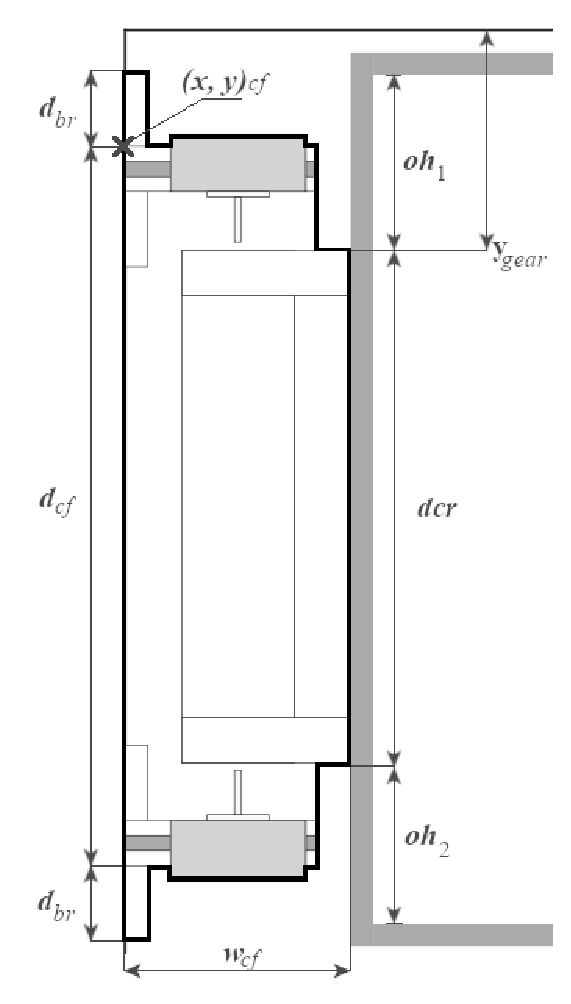
\includegraphics[width=.38\textwidth]{Elevator/CF.eps}
\end{wrapfigure}

In Fig.~\ref{img:dpDetailView} we consider a fragment of the
plan view focusing on the door pair --- notice that the car door and
the landing door $opening$ must be aligned. The drawing in 
Fig.~\ref{img:dpDetailView} represents a pair of telescopic
doors with 3 panels. The \emph{car door base point} $(x_{cd}, y_{cd})$
--- denoted as $(x,y)_{cd}$ in the plan view --- and the 
\emph{landing door base point} $(x_{ld}, y_{ld})$ --- denoted as 
$(x,y)_{ld}$ in the plan view --- are always at the top left corner 
of the corresponding structure.
The value of these coordinates represents a specific placement of the 
car/landing door pair. The landing door opening is surrounded by the 
\emph{frame}, i.e., the structure that surrounds the entrance to the 
car, with width $w_{frame}$. The total door width is the sum of two
parameters, the \emph{left axis} --- $la_{cd}$ and $la_{ld}$ for car
and landing door, respectively --- and the \emph{right axis} ---
$ra_{cd}$ and $ra_{ld}$ for car and landing door, respectively. Both
axes originate from the opening midpoint and, as shown in the drawing
of Fig.~\ref{img:dpDetailView}, in general they may not
coincide. Finally, $step_{cd}$ and $step_{ld}$ denote the depth of the
step in the car and landing door, respectively; $d_{step}$ is the
distance between car and landing doors.

%%
%% DECISION VARIABLES
%%
\begin{table}[t]
	\setlength{\tabcolsep}{20pt}
	\caption{\label{tab:variables} Explanation of the decision variables 
		involved in the design process} 
	\centering
	\begin{tabular}{rl}
		\toprule
		\textbf{Symbol} & \textbf{Description} \\
		\midrule
		$x_{cf}$, $y_{cf}$ 		& Car frame base point \\
		& coordinates \\
		& \\
		$x_{cd}$, $y_{cd}$ 		& Car door base point \\
		& coordinates \\
		$x_{ld}$, $y_{ld}$ 		& Landing door base point \\
		& coordinates \\
		& \\
		$x_{car}$, $y_{car}$ 	& Car base point coordinates \\
		$w_{car}$, $d_{car}$ 	& Car width and depth \\
		& \\
		\bottomrule
	\end{tabular}
\end{table}

\begin{table}[t]
	\setlength{\tabcolsep}{20pt}
	\caption{\label{tab:param} Explanation of the parameters 
		involved in the design process} 
	\centering
	\begin{tabular}{rl}
		\toprule
		\textbf{Symbol} & \textbf{Description} \\
		\midrule
		$x_{shaft}$, $y_{shaft}$ 	& Shaft base point
		coordinates \\
		$w_{shaft}$, $d_{shaft}$ & Shaft width and depth \\
		$red_{[N, E, S, W]}$ 	 & Distance between shaft and car \\
		& walls (North, East, South, West) \\
		$cwt_{[N, E, S, W]}$ 	 & Car wall thickness (North, East, \\
		& South, West) \\
		& \\
		
		$w_{cf}$ & Distance from $x_{cf}$ to the left car wall \\
		$d_{cf}$ & External distance between car frame rails \\
		$y_{gear}$ & Core gear placement with respect to the \\
		& car frame base point \\
		$d_{br}$ & External depth of the car frame bracket \\
		& from the base point \\
		$dcr$ & Distance between car rails\\
		$max_{oh}$ & Maximum car overhang that the car \\
		& frame is able to sustain \\
		$d_p$ & Diameter of the hydraulic cylinder barrell \\
		& \\
		
		$opening$ & Doors opening \\
		$la_{cd}$, $ra_{cd}$ & Left and right axis size (car door) \\
		$la_{ld}$, $ra_{ld}$ & Left and right axis size (landing door) \\
		$step_{cd}$ & Car door step \\
		$step_{ld}$ & Landing door step \\
		$d_{step}$ & Distance between doors \\
		$w_{frame}$ & Landing door external frame width \\
		& \\
		\bottomrule
	\end{tabular}
\end{table}

In Tables~\ref{tab:variables} and~\ref{tab:param} we summarize all 
the quantities involved in 
the configuration, separating decision variables (Table~\ref{tab:variables}) 
from parameters (Table~\ref{tab:param}) either related to the initial specification 
or extracted from the components database --- all quantities are in
millimeters. We introduced all the decision variables beforehand
with the exception of $(x_{car}, y_{car})$, i.e., the car base point
coordinates corresponding to the top-left internal edge of the car in
Fig.~\ref{img:planView}, and $w_{car}$ and $d_{car}$,
i.e., the width and depth of the car.
Concerning parameters, we consider four groups of them. The first group is 
related to shaft measurements and includes $w_{shaft}$ and $d_{shaft}$
--- width and depth of the shaft, respectively; also in this group
we have \emph{reductions} ($red_N$, $red_S$, etc.), i.e., the distance
between the car walls and the shaft, and \emph{car wall thicknesses}
($cwt_N$, $cwt_S$, etc.). For both such groups of parameters we have
four values  
($N$, $S$, $W$ and $E$) to account for different sizes on all
sides (top, bottom, left and right, respectively). The second group is
related to car frame dimensioning and includes $max_{oh}$, i.e., the
maximum overhang, and other parameters detailed in the table. The 
third group is related to doors --- no further parameters need to be
introduced in this group.  

\section{Constraints}
\label{sec:model_constraints}

% -------------------------------------------------------
% CONSTRAINTS: CAR FRAME
% -------------------------------------------------------
Having defined our decision variables and parameters, we proceed to
describe the (hard) constraints required to find feasible solutions,
divided into two groups related to car frame and doors respectively.
The constraints to place the car frame must take into account two main
issues. First, given the shape of the brackets, it is not possible 
to model the car frame as a simple rectangle in order to fit it with
the other components. Therefore the placement of the car frame is
computed by subtracting residuals from the total shaft
measures. Second, the placement of the car frame must take into
account its maximum overhang, i.e., the car cannot ``lean'' too much
outside the car frame core gear. The considerations above lead
to the following set of constraints:
\begin{equation}
\begin{cases}
y_{cf} - d_{br} \geq y_{shaft} \\
y_{cf} + d_{cf} + d_{br} \leq y_{shaft} + d_{shaft} \\
0 \leq y_{cf} + y_{gear} - y_{car} < max_{oh} \\ 
0 \leq y_{car} + d_{car} - y_{cf} - y_{gear} - dcr < max_{oh} \\
\end{cases}
\label{eq:CFConstr}
\end{equation}
The first two constraints are required to fit the
shape of the car frame, while the last two are required to satisfy the
requirement about the maximum overhang.

% -------------------------------------------------------
% CONSTRAINTS: DOOR PAIR
% -------------------------------------------------------
The constraints to place the car/landing door pair should
guarantee that both structures fit the shaft, that the actual
opening fits the car and that the landing door frame does not exceed
the shaft size. These requirements can be translated into the
following set of constraints:

\begin{equation}
\begin{cases}
x_{cd} \geq x_{shaft} \\
x_{ld} \geq x_{shaft} \\ 
x_{cd} + la_{cd} + ra_{cd} \leq x_{shaft} +
w_{shaft}\\
x_{ld} + la_{ld} + ra_{ld} \leq x_{shaft} + w_{shaft}\\
x_{cd} + la_{cd} - \frac{opening}{2} \geq x_{car}\\
x_{cd} + la_{cd} + \frac{opening}{2} \leq x_{car} + w_{car}\\
x_{ld} + la_{ld} + \frac{opening}{2} + w_{frame} \leq
x_{shaft} + w_{shaft}\\
\end{cases}
\label{eq:DoorConstr}
\end{equation}
The first four inequalities are required to guarantee that
the car and the landing door structures fit the shaft; then
we list two inequalities related to the car opening, and the last inequality
guarantees that the landing door frame size is adequate for the shaft.
In addition, the alignment of the landing door with respect to the car
door must be enforced with the following equality constraint:
\begin{equation}
x_{ld} = x_{cd} + la_{cd} - la_{ld}
\end{equation}
The placement of the car and landing door on the $y$ axis is also enforced
with equality constraints:
\begin{equation}
\label{eq:Doory}
\begin{cases}
y_{ld} = y_{shaft} + d_{shaft} - step_{ld}\\
y_{cd} = y_{ld} - d_{step} - step_{cd}
\end{cases}
\end{equation}
Further equality constraints are required to take into account
that the door placement over the $y$ axis, together with the car frame
and door selection, influences the car size as follows: 
\begin{equation}
\begin{cases}
x_{car} = w_{cf} + cwt_{W}\\ 
y_{car} = red_{N} + cwt_{N}\\ 
w_{car} = w_{shaft} - w_{cf} - cwt_{W} - cwt_{E} - red_{E}\\ 
d_{car} = d_{shaft} - red_{N} - cwt_{N} - cwt_{S} - H_{doors}\\
\end{cases}
\label{eq:CarConstr}
\end{equation}
where $H_{doors}$ stands for the total door occupancy over the $y$
axis computed as:
\begin{equation}
H_{doors} = step_{ld} + step_{cd} + d_{step}
\label{eqnDoorsH}
\end{equation}
Notice that when the car frame is positioned on the left hand side of the
elevator, its $x$ base coordinate $x_{cf}$ is always set to $0$.

Since the car door body may protrude over the car walls, in order to
minimize the risk of collision with other components, designers
must consider a safety margin. To
guarantee this requirement, specific non-overlapping constraints are 
implemented. For example, if we let $r$ be the security margin, the 
non-overlapping constraint relative to car frame and car door can be written 
as follows:
\begin{equation}
\label{eq:superpos}
x_{cd} - r \geq x_{cf} + w_{cf} \lor y_{cd} - r \geq y_{cf} + d_{cf}
\end{equation}

\begin{table}[t]
	\setlength{\tabcolsep}{20pt}
	\caption{\label{tab:constraints} Grouping of the constraints
		involved in the design process, separated by their 
		purpose}
	\centering
	\begin{tabular}{rll}
		\toprule
		\textbf{Class} & \textbf{Type} & \textbf{Number} \\
		\midrule
		Car Frame shape & $Inequality$ & 6 \\
		Doors shape & $Inequality$ & 7 \\
		& $Equality$ & 3 \\
		Car shape & $Equality$ & 4 \\
		Car Frame / Doors overlap & $Inequality$ & 2 \\
		Components selection (SMT) & $Implication$ & 308 \\
		\bottomrule 
	\end{tabular}
\end{table}

In Table~\ref{tab:constraints} we summarize the shape of our problem
by identifying the number of constraints and their type, based on their
purpose. The last element of the Table is related to the SMT encoding
where we use Boolean implications as constraints to choose the components.

\section{Objective}
\label{sec:objective}

In our process, we considered four design objectives that are the main
interests for technical engineers. The first is that the car frame 
should be aligned as much as possible to the center of the car on the 
$y$ axis --- i.e., considering Figure~\ref{img:planView}, the car frame
should appear vertically centered with respect to the car. The second 
objective regards doors positioning: in case of symmetric doors, i.e., 
the opening midpoint coincides with the door frame midpoint, the opening
of the car door should be aligned as much as possible to the center 
of the car on the $x$ axis; in case of asymmetric doors, then the 
opening should be as close as possible to the opposite side of the car
frame in order to minimize the chance of interference. 
Notice that in Figure~\ref{img:planView} we have a non-symmetric door, 
which is aligned to the right car wall. The third objective is that 
the car frame and the hydraulic cylinder should not be over-sized, 
and the opening of the car door should not be undersized during the 
components selection phase and finally, the last objective is to 
minimize the force exerted by the elevator on the car rails.

Here we describe the single objectives and we shape them as 
contributions to a cost function, mentioning the details of the 
parameters involved when necessary.  
The cost associated to car frame misalignment on the $y$ axis is 
expressed by the absolute value of the distance between the car frame
and the car axes. We define the car frame vertical axis $axisY_{cf}$ as 
the car frame vertical base point $y_{cf}$ plus half of the distance
between the car rails $dcr$
\begin{equation}
	\label{eq:cfaxis}
	axisY_{cf} = y_{cf} + \frac{dcr}{2}.
\end{equation}
The vertical car axis $axisY_{car}$ is defined as the car vertical base
point $y_{car}$ plus half of the car depth $d_{car}$: 
\begin{equation}
	\label{eq:caraxis}
	axisY_{car} = y_{car} + \frac{d_{car}}{2}.
\end{equation}
The difference between the terms (\ref{eq:cfaxis}) and
(\ref{eq:caraxis}) gives us the first contribution to the cost
function $c_{cf}$: 
\begin{equation}
	\label{eq:costoh}
	c_{cf} = |axisY_{cf} - axisY_{car}|
\end{equation} 
The second objective we consider is related to doors. In this case
we define the horizontal car axis $axisX_{car}$ as the horizontal car
base point $x_{car}$ plus half of the car width $w_{car}$:
\begin{equation}
	\label{eq:caraxis2}
	axisX_{car} = x_{car} + \frac{w_{car}}{2}
\end{equation}
The horizontal door axis $axisX_{door}$ is defined as the horizontal
door base coordinate $x_{cd}$ plus the length of its left axis $la_{cd}$:
\begin{equation}
	\label{eq:axisd}
	axisX_{door} = x_{cd} + la_{cd} 
\end{equation}
In the case of symmetric doors, good design practices suggest that 
$axisX_{door}$ and $axisX_{car}$ should be aligned. In the case of 
non-symmetric doors, it is preferable to have the door \textit{opening} 
as close as possible to the side of the car which is opposite to the 
car frame.
In a configuration like the one in Figure~\ref{img:planView}
we can define the base coordinate of such side as:
\begin{equation}
	\label{eq:xwall}
	x_{wall} = x_{car} + w_{car}
\end{equation}
To take into account the different arrangement of doors, we
introduce a binary variable, $\delta_{t}$, which is assigned to $1$
if the current door is a non-symmetric door and to $0$ otherwise.
We can then summarize the contribution to the cost function as:
\begin{equation}
	\label{eq:costdoor}
	\renewcommand{\arraystretch}{1.5}
	\begin{array}{lll}
		c_{door} = ( & (1 - \delta_{t})|axisX_{car} - axisX_{door}| + \\
		& \delta_{t}(x_{wall} - (axisX_{door} + \frac{opening}{2})) &)
	\end{array}
\end{equation}
The first contribution of (\ref{eq:costdoor}) is zero when $\delta_t = 1$, 
i.e, for non-symmetric doors we try to minimize the distance from 
the side of the elevator opposite to the car frame, whereas
when $\delta_t = 0$ we try to align the door and the car axes.
The third objective is related to the selection of the components, and
gives the guidelines for sizing the car frame, the doors and the cylinder.
The maximization of the door $opening$ leads to accessible elevators which 
are always considered a plus, whenever feasible; the minimization of the
car frame depth $dcr$ and the barrel diameter $d_p$ suggests components 
which are not over-sized, thus helping to keep costs at bay. These criteria 
can be translated into one additional contribution to the overall cost 
function defined as:
\begin{equation}
	\label{eq:choice}
	c_{size} = (dcr + d_{p} - opening)
\end{equation}
Finally, the last term to minimize is the sum of $F^x_{cr}$
and $F^y_{cr}$, i.e., the $x$ and $y$ components of
the force exerted on the car rails $F_{cr}$:
\begin{equation}
	\label{eq:cr}
	c_{cr} = F^x_{cr} + F^y_{cr}
\end{equation}
The computation of $F_{cr}$ is non-trivial and requires additional
equations and parameters that we briefly describe.
The components of $F_{cr}$ are obtained as
\begin{equation*}
	\label{eq:force}
	\begin{array}{rcl}
		F^x_{cr} & = & k \cdot g \cdot
		\frac{Q_x (Q + 75) + P_x \cdot car_W + cdP_x \cdot cd_W + cf_W 
			\cdot CF_x}{2 \cdot h}\\
		F^y_{cr} & = & k \cdot g \cdot
		\frac{Q_y (Q + 75) + P_y \cdot car_W + cdP_y \cdot cd_W}
		{2 \cdot h}
	\end{array}
\end{equation*}
where the parameters have the following meaning:
\begin{itemize}
	\item $k$ is a parameter depending on the kind
	of safety brakes installed;
	\item $g$ is the standard acceleration due to gravity;
	\item $Q$ is the car payload;
	\item $P_x$ and $P_y$ are the midpoint coordinates of the car;
	\item $Q_x$ and $Q_y$ are obtained through the equations
	\begin{equation*}
		\begin{array}{rcl}
			Q_x & = & max{\{P_x + \frac{w_{car}}{8}, P_x - \frac{w_{car}}{8}\}} \\
			Q_y & = & max{\{P_y + \frac{d_{car}}{8}, P_y - \frac{d_{car}}{8}\}};
		\end{array}
	\end{equation*}
	\item $car_W$ is the car weight;
	\item $cdP_x$, $cdP_y$ are the coordinates of the center of gravity of
	the car door;
	\item $cd_W$ is the car door weight and $cf_W$ is the car frame weight;
	\item $CF_x$ is a coefficient computed as
	\begin{equation*}
		CF_x = 1.5 \cdot\frac{w_{cf}}{2}
	\end{equation*}
	where $w_{cf}$ is the distance from the car frame base point to to
	the left car wall;
	\item $h$ is the distance between guide shoes, i.e., the supports 
	which slide on the car rails.
\end{itemize}

